\documentclass[11pt]{article}
\usepackage[margin=0.75in]{geometry}
\usepackage{amsmath,amsfonts}
\usepackage{enumitem}
\usepackage{tikz}
\usepackage{pgfplots}
\usepackage{soul}

\usepackage{multicol}

\newcommand{\ds}{\displaystyle}
\newcommand{\N}{\mathbb{N}}
\newcommand{\R}{\mathbb{R}}
\newcommand{\C}{\mathbb{C}}
\newcommand{\re}{\operatorname{Re}}
\newcommand{\im}{\operatorname{Im}}
\newcommand{\on}{\operatorname}
\newcommand{\Log}{\on{Log}}
\newcommand{\Arg}{\on{Arg}}


\begin{document}
\newcounter{enumCount}
\pagestyle{empty}
\subsection*{Math 444 - Homework 8 \hfill Name: \underline{\hspace*{2in}}}
\noindent

\begin{enumerate}

\item Show that $F(z) = \frac{i}{2} \Log(z + i) - \frac{i}{2} \Log(z- i)$ is an antiderivative of $\dfrac{1}{1+z^2}$ on the open right half-plane (the set of $z \in \C$ such that $\re(z) > 0$).
\vfill  

\item The standard parametrization of the unit circle is $z = e^{it}$. In this parametrization, what are the differentials $dx$, $dy$, and $dz$?  
\vfill


\item Use Green's theorem to compute $\ds \oint_C y^2 \, dx - x^2 \, dy$ where $C$ is the square with vertices $(0,0)$, $(1,0)$, $(1,1)$ and $(0,1)$. 
\vfill

\newpage
\item Find a vector field $\mathbf{F}: \R^2 \rightarrow \R^2$ for which $\on{curl} F = 1$ everywhere on $\R^2$. Hint: Recall that  
$$\ds \on{curl} \mathbf{F} = \frac{\partial Q}{\partial x} - \frac{\partial P}{\partial y}$$
if $\mathbf{F}(x,y) = (P(x,y),Q(x,y))$. Choose the simplest functions $P$ and $Q$ that you can think of to make the curl equal one everywhere. There is more than one correct answer.
\vfill

\item Use your answer to the last problem to calculate the area of the region $D$ enclosed by the curve $(\sin 2t, \sin t)$ with $0 \le t \le \pi$.  Hint: Use Green's theorem to calculate the line integral $\ds \oint_C P dx + Q dy$ in order to find $\ds \iint_D 1 \, dA$.  
\begin{flushright}
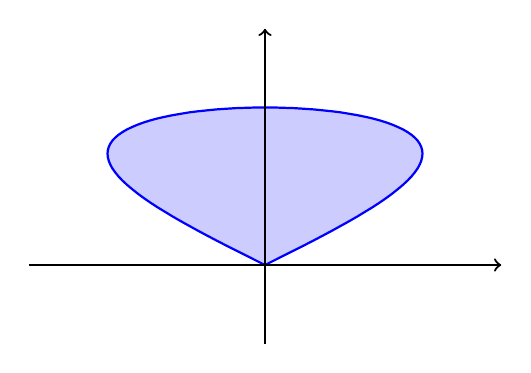
\begin{tikzpicture}[scale=2]
\filldraw[fill=blue!20,draw=blue,thick] (0.0,0.0)--(0.0628,0.0314)--(0.125,0.0628)--(0.187,0.0941)--(0.249,0.125)--(0.309,0.156)--(0.368,0.187)--(0.426,0.218)--(0.482,0.249)--(0.536,0.279)--(0.588,0.309)--(0.637,0.339)--(0.685,0.368)--(0.729,0.397)--(0.771,0.426)--(0.809,0.454)--(0.844,0.482)--(0.876,0.509)--(0.905,0.536)--(0.93,0.562)--(0.951,0.588)--(0.969,0.613)--(0.982,0.637)--(0.992,0.661)--(0.998,0.685)--(1.0,0.707)--(0.998,0.729)--(0.992,0.75)--(0.982,0.771)--(0.969,0.79)--(0.951,0.809)--(0.93,0.827)--(0.905,0.844)--(0.876,0.861)--(0.844,0.876)--(0.809,0.891)--(0.771,0.905)--(0.729,0.918)--(0.685,0.93)--(0.637,0.941)--(0.588,0.951)--(0.536,0.96)--(0.482,0.969)--(0.426,0.976)--(0.368,0.982)--(0.309,0.988)--(0.249,0.992)--(0.187,0.996)--(0.125,0.998)--(0.0628,1.0)--(1.22e-16,1.0)--(-0.0628,1.0)--(-0.125,0.998)--(-0.187,0.996)--(-0.249,0.992)--(-0.309,0.988)--(-0.368,0.982)--(-0.426,0.976)--(-0.482,0.969)--(-0.536,0.96)--(-0.588,0.951)--(-0.637,0.941)--(-0.685,0.93)--(-0.729,0.918)--(-0.771,0.905)--(-0.809,0.891)--(-0.844,0.876)--(-0.876,0.861)--(-0.905,0.844)--(-0.93,0.827)--(-0.951,0.809)--(-0.969,0.79)--(-0.982,0.771)--(-0.992,0.75)--(-0.998,0.729)--(-1.0,0.707)--(-0.998,0.685)--(-0.992,0.661)--(-0.982,0.637)--(-0.969,0.613)--(-0.951,0.588)--(-0.93,0.562)--(-0.905,0.536)--(-0.876,0.509)--(-0.844,0.482)--(-0.809,0.454)--(-0.771,0.426)--(-0.729,0.397)--(-0.685,0.368)--(-0.637,0.339)--(-0.588,0.309)--(-0.536,0.279)--(-0.482,0.249)--(-0.426,0.218)--(-0.368,0.187)--(-0.309,0.156)--(-0.249,0.125)--(-0.187,0.0941)--(-0.125,0.0628)--(-0.0628,0.0314)--(0,0);
\draw[thick,->] (-1.5,0) -- (1.5,0);
\draw[thick,->] (0,-0.5) -- (0,1.5);
\end{tikzpicture}
\end{flushright}
~\\

\item Let $f(z) = \ds \frac{z}{z^2 - 5z + 4}$ and $g(z) = \ds \frac{z^2 + 3z - 4}{e^{2z-8}}$.  Let $C$ be the circle centered at $z = 4$ with radius 2, oriented clockwise. One of the integrals $\ds \oint_C f(z) \, dz$ or $\ds \oint_C g(z) \, dz$ is zero.  Without calculating anything, explain which integral must be zero, and why. 
\vfill 


\end{enumerate}
\end{document}
